\documentclass{beamer}
\usepackage[french]{babel}
\usepackage{hyperref}
\definecolor{links}{HTML}{2A1B81}
\hypersetup{colorlinks,linkcolor=,urlcolor=links}
\usepackage{graphicx}
\usepackage{amsmath,amssymb}
\usepackage{tabularx}
\usepackage{booktabs}
\usepackage[compatibility=false]{caption}
\usepackage[toc,page]{appendix}
\usepackage{minted}
\usepackage{xspace}

\makeatletter
  \def\beamer@calltheme#1#2#3{%
    \def\beamer@themelist{#2}
    \@for\beamer@themename:=\beamer@themelist\do
    {\usepackage[{#1}]{\beamer@themelocation/#3\beamer@themename}}}

  \def\usefolder#1{
    \def\beamer@themelocation{#1}
  }
  \def\beamer@themelocation{}

\patchcmd{\minted@colorbg}{\noindent}{\medskip\noindent}{}{}
\apptocmd{\endminted@colorbg}{\par\medskip}{}{}
\makeatother

\newcolumntype{Y}{>{\centering\arraybackslash}X}

\usefolder{../theme}
\usetheme[numbering=fraction,block=fill,progressbar=frametitle]{metropolis} %Use metropolis theme

\definecolor{bg}{rgb}{0.95,0.95,0.95}
\setminted{bgcolor=bg,fontsize=\scriptsize,autogobble,mathescape,breaklines,tabsize=2}
\setmintedinline{breaklines,autogobble,fontsize=\scriptsize}
\setbeamersize{text margin left=8pt,text margin right=8pt}
\setbeamercovered{transparent}

\begin{document}

\title[C++]{Introduction à la programmation en C++}
\author[nicolas.audebert@onera.fr]{Nicolas Audebert}
\setmainfont{Fira Sans}


\AtBeginSection[]{
  \begin{frame}{Plan de la séance}
  \small \tableofcontents[currentsection]
  \end{frame}
}

\newcommand\cppi[1]{\mintinline{cpp}{#1}}
\newcommand\cpp[1]{%
  \begin{minted}{cpp}
  #1
  \end{minted}
}%

\subtitle{Fichiers séparés - Opérateurs}
\date[6 oct. 2017]{Vendredi 13 octobre 2017}
\maketitle

\begin{frame}{Avant toute chose}
  \begin{alertblock}{Rendus de TP et des exercices}
  Les rendus se font sur \href{https://educnet.enpc.fr}{\textbf{Educnet}}.
  \begin{enumerate}
    \item Le code rendu \textbf{doit compiler}.
    \item Le code rendu doit \textbf{être propre} (indentation, noms de variables clairs).
    \item Le code rendu doit \textbf{être commenté} (réponses aux questions, fonctionnement du code).
    \item Rassembler le code dans une seule archive (\texttt{.zip}, \texttt{.rar}, \texttt{.tar.gz}, etc.).
  \end{enumerate}
  \end{alertblock}
\end{frame}

\section{Rappels}

\begin{frame}[fragile=singleslide]
	\frametitle{Les structures}
	\begin{block}{Définition}
		Les \textbf{structures} C++ permettent de regrouper des variables hétérogènes dans un ensemble cohérent. Une structure définit un nouveau \textbf{type}.
	\end{block}

\begin{minipage}{0.47\linewidth}
		\begin{minted}{cpp}
struct Point{
	double x,y;
};

struct Cercle{
    Point centre;
    double rayon;
    Color couleur;
};

Cercle c;
c.centre.x = 0.5;
c.couleur = RED;
		\end{minted}
\end{minipage}
\begin{minipage}{0.47\linewidth}
		\begin{minted}{cpp}
Point pt;
pt.x = pt.y = 5.5;
c.centre = pt;

Point p1={1,2}, p2;
p2 = p1;

// Tableau de cercles
Cercle liste_cercles[10];
for(int i=0; i<10; i++){
	liste_cercle[i] = c;
}
		\end{minted}
\end{minipage}
\end{frame}

\section{Organiser son code}

\begin{frame}
\frametitle{Fichiers séparés\dots}

Jusqu'ici, tout le code est organisé un seul fichier qui contient :
\begin{itemize}
	\item une fonction \mintinline{cpp}{main} (le point d'entrée du programme),
    \item des définitions de fonction,
    \item des définitions de structure.
\end{itemize}

\begin{block}{En pratique}
Structurer son code dans plusieurs fichiers permet de :
\begin{itemize}
	\item mieux organiser le programme (plus lisible, regroupements par modules),
    \item partager ses fonctions et de les réutiliser dans plusieurs projets,
    \item accélérer la compilation des gros projets.
\end{itemize}
\end{block}
\end{frame}

\subsection{Plusieurs fichiers sources}

\begin{frame}[fragile=singleslide]
\frametitle{Multiples fichiers sources}
Ce qu'on aimerait faire, c'est pouvoir définir une fonction dans un fichier et la réutiliser dans un autre.
  \begin{minipage}{0.49\textwidth}
  	\begin{minted}{cpp}
	// fichier1.cpp
	
	int ma_fonction(int var){
		...
		autre(var);
		// ERREUR : autre est inconnue !
		...
    }
	\end{minted}
  \end{minipage}
  \begin{minipage}{0.49\textwidth}
	\begin{minted}{cpp}
	// fichier2.cpp
	
	void autre(int arg){
		...
		...
	}
	\end{minted}
  \end{minipage}
\begin{alertblock}{Attention}
Pour pouvoir utiliser une fonction, il faut qu'elle soit connue dans le fichier où on l'utilise.
\end{alertblock}
\end{frame}

\begin{frame}[fragile=singleslide]
\frametitle{Multiples fichiers sources}
  \begin{minipage}{0.49\textwidth}
  	\begin{minted}{cpp}
	// fichier1.cpp
	
	// Signature de autre_fonction
	void autre(int arg);
	
	int ma_fonction(int var){
		...
		autre(var); // OK
		...
	}
	\end{minted}
  \end{minipage}
  \begin{minipage}{0.49\textwidth}
	\begin{minted}{cpp}
	// fichier2.cpp
    
    void autre(int arg){
        ...
    }
	\end{minted}
  \end{minipage}
  
  \begin{block}{Solution}
		On déclare la fonction dans le fichier qui souhaite l'utiliser pour signifier au compilateur que la fonction existe.
	\end{block}
\end{frame}

\begin{frame}{Pourquoi ?}

La production d'un exécutable à partir du code source C++ se réalise en deux étapes :
\begin{enumerate}
	\item<1->La compilation (transforme le code en fichiers objets)
    \item<2>L'édition des liens (transformes les fichiers objets en exécutable)
\end{enumerate}

\begin{center}
	\includegraphics<1>[width=0.7\linewidth]{images/compile_01.pdf}
	\includegraphics<2>[width=0.7\linewidth]{images/compile_02.pdf}
\end{center}

\end{frame}

\begin{frame}{Oui mais\dots pourquoi ?!}

Ce fonctionnement présente deux intérêts :
\begin{itemize}
	\item La compilation est plus rapide : on ne recompile que les fichiers \texttt{.cpp} qui ont été modifiés.
    \item On peut créer et utiliser des librairies : des fichiers précompilés et réutilisés dans notre propre code (exemple: Imagine++).
\end{itemize}
\end{frame}

\begin{frame}[fragile]
\frametitle{CMake}
CMake contrôle le compilateur et l'éditeur de liens.

\begin{minted}{cmake}
cmake_minimum_required(VERSION 2.6)
# On indique à l'éditeur de liens où trouver Imagine++
file(TO_CMAKE_PATH "$ENV{IMAGINEPP_ROOT}/CMake" p)
# On indique que Imagine++ est REQUIS pour compiler
find_package(Imagine REQUIRED)

# On nomme le projet
project(Mon_projet_cpp)

# On indique quels sont les fichiers sources à compiler
# On peut compiler plusieurs programmes différents dans un
# même projet !
add_executable(Mon_executable
 fichier1.cpp fichier2.cpp fichier3.cpp ...
)
# On indique quels sont les modules Imagine++ utilisés par
# les différents exécutables
ImagineUseModules(Mon_executable Graphics)
\end{minted}

\end{frame}


\begin{frame}
	\frametitle{Ajouter un fichier dans un projet existant}
	
	\begin{block}{Solution pour tous les IDEs}
		\begin{enumerate}
			\item créer le fichier dans le même dossier que les autres,
			\item modifier le CMakeLists.txt avec un éditeur de texte :
			ajouter le nom du fichier
			\item recompiler le programme dans l'IDE.
		\end{enumerate}
	\end{block}
	
\end{frame}

\begin{frame}
	\frametitle{Ajouter un fichier dans un projet existant}
	
	\begin{block}{Solution pour QtCreator}
		Dans QtCreator :
		\begin{enumerate}
		\item ouvrir le menu \texttt{File/New File or Project} ou faire \texttt{Ctrl+N}, choisir \textit{C++ Source File}. \textbf{Attention : mettre le fichier dans le dossier des sources},
		\item rajouter ce fichier dans le \texttt{CMakeLists.txt},
		\item recompiler le programme dans QtCreator.
		\end{enumerate}
	\end{block}
	
\end{frame}

\subsection{Les fichiers d'en-tête}

\begin{frame}
\frametitle{Les fichiers d'en-tête}

\begin{exampleblock}{Constat}
\begin{itemize}
	\item Pénible de recopier toutes les déclarations dans tous les fichiers \textbf{.cpp},
	\item Pas de partage des structures de cette façon.
\end{itemize}
\end{exampleblock}

\begin{block}{Solution}
	Mettre toutes les \textbf{déclarations} et les \textbf{structures} dans des \textbf{fichiers d'en-tête} (\textit{header}) repérés par l'extension \textbf{.h}
\end{block}
\end{frame}

\begin{frame}[fragile=singleslide]
\frametitle{Mise en \oe{}uvre}

\begin{minipage}{0.49\textwidth}
\begin{minted}{cpp}
// source.cpp

#include "auxiliaire.h"
// similaire au import Python

int ma_fonction(int var){
	...
	autre(var);
	...
}
\end{minted}
\end{minipage}
\begin{minipage}{0.48\textwidth}
\begin{minted}{cpp}
// auxiliaire.h
// Signature
void autre(int var);

struct Vect{ ... };

// auxiliaire.cpp
#include "auxiliaire.h"

// Définition
void autre(int var){...}
\end{minted}
\end{minipage}

\begin{block}{Note}
Jusqu'à présent, les fonctions externes au projet étaient incluses grâce à la directive \texttt{\#include<...>}. Il s'agit en fait de headers externes pour différents librairies (librairie standard \texttt{std}, librairie Imagine++, \dots).
\end{block}

\end{frame}

\begin{frame}
\frametitle{Ajouter un fichier d'en-tête dans un projet}

\begin{block}{Méthode générique}
	Exactement comme pour les \texttt{.cpp}.
\end{block}

\begin{block}{QtCreator}
	Idem, mais il faut créer un \textit{C++ Header File}.
\end{block}

\end{frame}

\begin{frame}[fragile=singleslide]
\frametitle{Inclusions mutuelles}

En pratique, la directive \texttt{include} ne fait que copier et coller l'en-tête dans le fichier source et rien n'empêche les inclusions mutuelles :

\begin{minipage}{0.47\linewidth}
	\begin{minted}{cpp}
		// fichier1.h
		
		#include "fichier2.h"
		
		int function(int var);
	\end{minted}
\end{minipage}
\begin{minipage}{0.47\linewidth}
	\begin{minted}{cpp}
		// fichier2.h
		
		#include "fichier1.h"
		
		void aux(double arg);
	\end{minted}
\end{minipage}

	\begin{alertblock}{Attention}
		Boucle dans les inclusions $\rightarrow$ compilation impossible et plantage.
	\end{alertblock}
\end{frame}

\begin{frame}[fragile=singleslide]
	\frametitle{Se protéger des inclusions mutuelles}
    
\begin{minipage}{0.49\linewidth}
	La version classique :
    \begin{minted}{cpp}
// fichier1.h
#ifndef NOM_UNIQUE
#define NOM_UNIQUE

#include "fichier2.h"

int function(int var);

#endif
	\end{minted}
\end{minipage}
\begin{minipage}{0.49\linewidth}
	La version moderne :
    \begin{minted}{cpp}
// fichier1.h
#pragma once

#include "fichier2.h"

int function(int var);
	\end{minted}
\end{minipage}

\begin{block}{Intérêt}
Dans les deux cas, les directives du pré-processeur (préfixées par \texttt{\#}) permettent de s'assurer qu'un fichier est inclus au plus une fois.
\end{block}

\end{frame}

\section{Les opérateurs}

\begin{frame}
\frametitle{Opérateurs}
Les \textbf{opérateurs} définissent le comportement de certains signes de ponctuation ou mathématiques : 
\begin{itemize}
\item +~~~-~~~/~~~*~~~=~~~\dots
\end{itemize}

Il est possible de redéfinir ces opérateurs pour les utiliser avec les structures que l'on a créé.
\end{frame}

\begin{frame}[fragile=singleslide]
\frametitle{Exemple}
	\begin{minted}{cpp}
	struct Point {
		double x, y;
	}
	Point v1 = {0,0}, v2 = {1,5};
    \end{minted}
    Pour l'instant, on doit écrire :
    \begin{minted}{cpp}	
	// Addition
	Point v3 = {v1.x+v2.x, v1.y+v2.y};
	// Produit scalaire
	double s = v1.x*v2.x + v1.y*v2.y;
    \end{minted}
    Mais on aimerait :
    \begin{minted}{cpp}	
	Point v3 = v1 + v2;
	double s = v1 * v2;
    \end{minted}
\end{frame}

\begin{frame}[fragile=singleslide]
\frametitle{Implémentation}
\begin{minted}{cpp}
// opérateur + sur des vecteurs
Point operator+(Point vA, Point vB){
    Vect v = {vA.x+vB.x, vA.y+vB.y};
    return v;
}

// opérateur * sur des vecteurs
double operator*(Point vA, Point vB){
    return vA.x*vB.x + vA.y*vB.y;
}

Point v1 = {1, 2}, v2 = {5, 5};
// addition de deux vecteurs
Point v3 = v1+v2;
// produit scalaire
double s = v1*v2;
\end{minted}
\end{frame}

\begin{frame}[fragile=singleslide]
\frametitle{Surcharge des opérateurs}

\begin{minted}{cpp}
// opérateur * pour deux vecteurs
double operator*(Point vA, Point vB){
    return vA.x*vB.x + vA.y*vB.y;
}

// opérateur * vecteur et réel
Point operator*(Vect vA, double alpha){
    Point v = {alpha*v.x, alpha*v.y};
    return v;
}

Point v1 = {1, 2}, v2 = {5, 5};

// produit scalaire
double s = v1*v2;

// multiplication par un réel
double m = 5.5;
Point v3 = v1 * m;
\end{minted}
\end{frame}

\begin{frame}[fragile=singleslide]
\frametitle{Surcharge des opérateurs}
\begin{alertblock}{Attention}
L'ordre des arguments et important : \texttt{v1 * m} est différent de \texttt{m * v1}. La commutativité doit être explicitement définie.
\end{alertblock}
\begin{minipage}{0.47\linewidth}
\begin{minted}{cpp}
// opérateur * vecteur et réel
Point operator*(Point vA, double alpha){
    Point v = {alpha*v.x, alpha*v.y};
    return v;
}

// opérateur * vecteur et réel
Point operator*(double alpha, Point vA){
    return v*alpha;
}
\end{minted}
\end{minipage}
\hfill
\begin{minipage}{0.47\linewidth}
\begin{minted}{cpp}
Point v1, v2;
...

// multiplication par un réel
double m = 5.5;

Point v3 = v1*m;

Point v4 = m*v2;
\end{minted}
\end{minipage}
\end{frame}


\section{Le TP du jour}

\begin{frame}
\frametitle{Le TP du jour}
\begin{minipage}{0.45\textwidth}
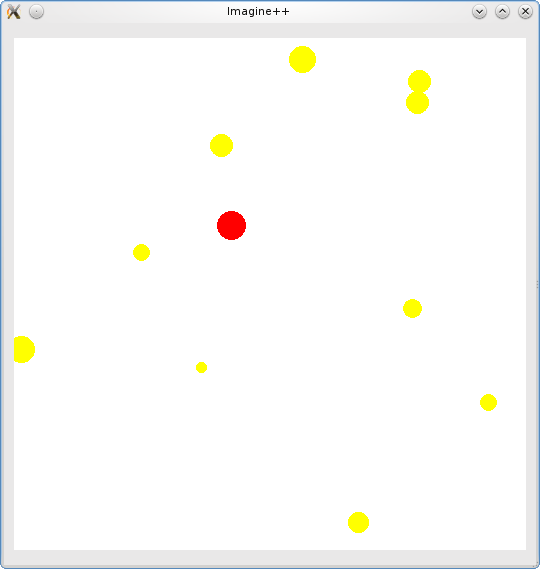
\includegraphics[width=\textwidth]{images/gravit.png}
\end{minipage}
\hfill
\begin{minipage}{0.48\textwidth}
On continue le TP "Gravitation".

\begin{enumerate}
\item Finir le TP de la séance précédente,
\item Organiser son code dans plusieurs fichiers,
\item Utiliser des opérateurs personnalisés pour les calculs.
\end{enumerate}
\end{minipage}
\end{frame}

\end{document}


